\documentclass{article}
\usepackage[utf8]{inputenc}
\usepackage{graphicx}
\usepackage{parskip}
\title{Introducción a la Biomecanica}
\author{Angel Gonzalez Melendres \\Alfredo Cárdenas Mena\\Aarón Lozano A\\Daniel Garcia R\\Angel Mario Acalá R}
\date{22 Agosto 2022} 

\begin{document}

\maketitle

\tableofcontents

\section{Introducción}

Al concepto de biomecánica se le conoce como el estudio de la estructura, función y movimiento de los aspectos mecánicos de los sistemas biológicos, utilizando los métodos de la mecánica. En simples palabras la biomecánica es una rama de la biofísica que tiene por objeto el estudio de las estructuras de carácter mecánico que existen en los seres vivos, fundamentalmente del cuerpo humano. Esta área de conocimiento se apoya en diversas ciencias biomédicas, utilizando los conocimientos de la mecánica, la ingeniería, la anatomía, la fisiología y otras disciplinas, para estudiar el comportamiento del cuerpo humano y resolver los problemas derivados de las diversas condiciones a las que puede verse sometido. 

La biomecánica juega un papel muy importante en las prótesis, ya que las prótesis completas, gracias a su diseño, deben ser capaces de contrarrestar o anular todas las cargas que actúen sobre ellas. Hoy se puede considerar que la biomecánica de las prótesis consiste en su funcionamiento basado en tres principios: retención, soporte y estabilidad. 

\section{Desarrollo}

\subsection{Mecanica}
Una de las ramas de la física muy conocida y estudiada es la mecánica, esta rama de la física estudia y describe el movimiento de los cuerpos, además de su evolución en el tiempo bajo la acción de distintas fuerzas que interactúan en dicho cuerpo. Para comprender todo este tema de estudio sobre la mecánica se comienza con la definición de las distintas magnitudes que afectan el movimiento de los objetos, entres estas magnitudes están el desplazamiento, el tiempo, la velocidad, la aceleración, la masa y la fuerza. 

La mecánica es tan extensa que se puede dividir en distintas secciones pero una de las que vamos hablar principalmente es la mecánica clásica. La mecánica clásica está formada por áreas de estudio que van desde la mecánica del sólido rígido y otros sistemas mecánicos con un número finito de grados de libertad, como la mecánica de medios continuos (sistemas con infinitos grados de libertad). 

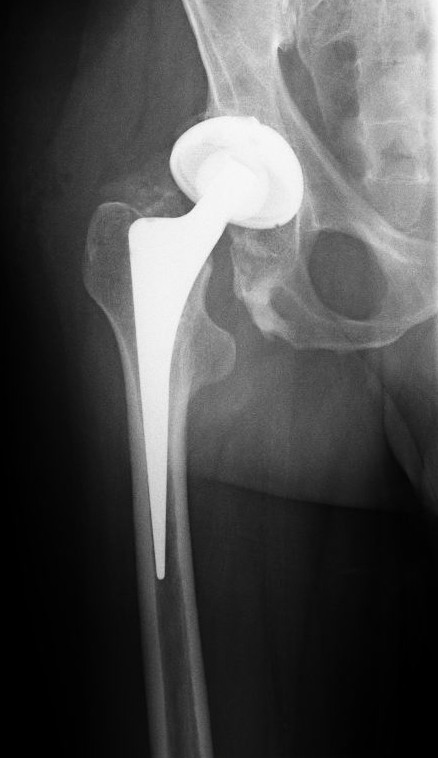
\includegraphics [scale=.35]{Investigación de la Biomecanica/Imagen1.jpg}

Ha sido de gran utilidad para el desarrollo humano debido a la gran variedad de aplicaciones de los conocimientos que se obtienen de la mecánica ya que gracias a esta se han realizado construcciones con movimientos mecánicos facilitando distintos procesos que realizan las personas, estas aplicaciones que nos ofrecen son la razón por la que el estudio de la mecánica es abarcado por distintos ámbitos como por ejemplo en la ingeniería, en la mecánica automotriz e incluso en la medicina.

La mecánica es tan extensa que se relaciona con otras áreas de estudio y una de las que nos interesa es la biomecánica la cual es una disciplina científica que tiene por objeto el estudio de las causas mecánicas y biológicas de los movimientos de los seres vivos, para este propósito se apoya en conocimientos de mecanica, ingenieria, anatomía y fisiología estudiando así como se comporta el cuerpo humano y los problemas que surgen de las condiciones a las que se ve sometido. El objeto de conocimiento de la biomecánica son: las acciones motoras del hombre como sistema de movimientos activos y las posiciones de su cuerpo estrechamente relacionadas entre sí.

\subsection{Protesis}
Una prótesis es un sustituto artificial de una parte del cuerpo faltante (tanto en singular como en plural; se llama prótesis). 


En ocasiones, se debe extirpar una parte del cuerpo si se encuentra cáncer en ella. Además, a veces recibir tratamiento podría resultar en la caída del cabello. En cualquier caso, se puede usar una prótesis para ayudar con la apariencia después de una cirugía u otro tratamiento para el cáncer. Esto puede ayudar a que una persona luzca como si la parte del cuerpo nunca hubiera sido extirpada o como si esa caída del cabello no hubiera ocurrido. Además, ayuda a que la persona se sienta mejor y funcione lo más naturalmente posible.

Una prótesis puede ser cosmética, funcional o ambas. La prótesis cosmética generalmente se diseña con el único propósito de hacer que la extremidad luzca natural y proporciona poca o ninguna funcionalidad. La prótesis funcional, por otro lado, puede ayudar a un amputado a realizar ciertas tareas que son desafiantes o imposibles después de la pérdida de una extremidad. Sin embargo, normalmente ofrece poco o ningún disfraz cosmético.


\textbf{Tipos de protesis: } 

\textbf{-Cadera:} Una prótesis de titanio, con una cabeza cerámica y copa acetabular de polietileno. El reemplazo total de cadera, conocido en términos médicos como artroplastia de cadera, consiste en la cirugía ortopédica que busca reemplazar de forma total la articulación de la cadera con un implante artificial llamado prótesis.

\textbf{Rodilla:}La prótesis de rodilla permite al paciente recuperar la movilidad y estabilidad de la articulación

El motivo más común por el que se coloca una prótesis es a causa de una artrosis de rodilla (gonartrosis), que va dañando la articulación. Pero también algunas fracturas en que hay un gran daño del hueso subcondral o determinados tumores óseos hacen necesario un implante o prótesis de rodilla.

\textbf{Hombro:} Los problemas degenerativos del hombro son una de las principales causas de incapacidad laboral. Para los pacientes supone un problema de salud equiparable, en su percepción de enfermedad, a la insuficiencia cardíaca o la diabetes. La prótesis de hombro, que podría ser una solución para muchos enfermos, es desconocida para gran parte de la población.

La prótesis de hombro, artroplastia de hombro o sustitución protésica de hombro es un procedimiento quirúrgico mediante el cual se sustituye la articulación glenohumeral (la articulación entre la cabeza del húmero y la escápula) por un implante protésico. Este procedimiento está indicado fundamentalmente en casos de artrosis evolucionada o de artritis severa de hombro (como en la artritis reumatoide) para controlar el dolor y recuperar la funcionalidad perdida; y también tras algunas fracturas de hombro proximal en las que la reconstrucción quirúrgica no es posible.

\textbf{Brazo:} Una prótesis de extremidad superior se refiere a un dispositivo fabricado artificialmente que sirve como sustituto de brazo parcial o totalmente perdido debido a un accidente, lesión, enfermedad o defecto congénito. Vienen en diferentes formas, tamaños y diseños. Un brazo protésico comprende típicamente ejes, encajes y componentes para imitar la unión del miembro a una articulación o rótula. Se puede fijar al cuerpo mediante el uso de cables.

\textbf{Mano:} Existen muchos tipos de protesis de mano:
   Mecánica, electrica, neumatica, hibrida

   Todas con distintos funcionamientos pero llegando a la mismo objetivo que es dar uso de una mano

\textbf{Pierna:}Una prótesis de pierna es un aparato diseñado para reemplazar artificialmente la extremidad inferior de un cuerpo humano, pudiendo suplantar de forma estética como funcional la ausencia de una pierna.

Estos aparatos tienen la finalidad de restablecer el soporte, equilibrio y la fuerza requerida para que las personas con amputaciones de pierna por accidentes o enfermedad puedan volver a ponerse de pie y caminar, recuperando su calidad de vida y pudiendo retomar las actividades que desempeñaban con anterioridad.

Las prótesis se diagnostican y fabrican de forma personalizada dependiendo del tipo de amputación, forma del muñón, necesidades y fuerza física de la persona.

\subsection{Biomecánica en las prótesis}
Tenemos que conseguir los siguientes objetivos:

• Aceptación por parte del paciente: estética y funcionalmente.

• Tolerancia de las estructuras: osteomucosas, dentoperiodontales, articulares.

• No introducir elementos iatrogénicos: para conseguir supervivencia a largo plazo.

Si conseguimos todo esto, nuestra prótesis conseguirá un éxito asegurado.

La biomecánica es una ciencia aplicada que estudia las leyes que siguen las interacciones entre los materiales y la vida. Es la interacción entre las estructuras anatómicas de soporte y retención y los elementos protésicos, frente a las fuerzas generadas durante los movimientos funcionales.

Cuando la protesis está instalada y durante la función, van a producirse una serie de fuerzas que generarán diversos movimientos sobre la prótesis y sus elementos (en los 3 planos del espacio), especialmente sobre las bases.

Estos movimientos van a originar unas fuerzas que a su vez van a ser transmitidas a los tejidos de soporte a través de los elementos que componen la PPR

Las fuerzas van a depender de una serie de factores:

•\text{Magnitud}: la cantidad de fuerza que se genera.

•\text{Dirección}: no es lo mismo una fuerza horizontal que una vertical que una oblicua.

•\text{Duración}: no es lo mismo durar 24h que 1 minuto.

•\text{Frecuencia}: las veces que se aplica la fuerza influye.

Existen distintos tipos de fuerzas que pueden actuar sobre las prótesis como consecuencia del desarrollo de las funciones orales de los pacientes. Las fuerzas de tracción son cargas verticales que actúan en sentido opuesto al de inserción de las prótesis. Las fuerzas compresivas son cargas verticales que actúan en el sentido de inserción de la prótesis. Las fuerzas horizontales son cargas latero-laterales, de flexión y rotación. En la práctica, las fuerzas que actúan sobre las prótesis son cargas complejas de cuya descomposición vectorial se obtienen los componentes de fuerza anteriormente descritos. Las prótesis completas, gracias a su diseño, deben ser capaces de contrarrestar o anular todas las cargas que actúen sobre ellas. Hoy se puede considerar que la biomecánica de las prótesis consiste en su funcionamiento basado en tres principios: retención, soporte y estabilidad.

La retención es la propiedad que tienen las prótesis para que no se produzca su extrusión, y por tanto su desestabilización en el sentido vertical de inserción; es decir, es la capacidad de dichas prótesis de oponerse a las fuerzas de tracción.

La estabilidad es la propiedad que tienen las prótesis para conservar su posición de reposo o de volver a ella después de haber realizado movimientos funcionales; es decir, es la capacidad de dichas prótesis de oponerse a las fuerzas horizontales, de cizallamiento y rotación.

Los principales factores que permiten lograr retención, soporte y estabilidad en una prótesis son la adhesión, la presión atmosférica y la estabilidad oclusal.

El diseño de una prótesis deberá ir dirigido a minimizar los factores que comprometan la retención, estabilidad y soporte adecuados para un correcto funcionamiento biomecánico de la rehabilitación durante el desarrollo de las funciones orales. De ahí la importancia de conocer las estructuras anatómicas bucofaciales, las fuerzas que actuarán sobre las prótesis, y la forma de aprovechar o evitar elementos favorecedores o comprometedores del buen funcionamiento de las restauraciones.

Por todo ello, la sistematización en la práctica clínica, no debe hacernos olvidar los principios básicos que deben guiar el diseño de una prótesis para controlar y manejar a nuestro favor los factores biomecánicos de los que dependerá en buena medida el éxito, confort y durabilidad de nuestros tratamientos.

\section{Conclusión}
La biomecanica  abarca una gran cantidad de  distintas areasco   como son la ingenieria, la fisiologia estas juegan un papel muy importante porque facilita la comprehension de la mecanica de los cuerpos humanos asi como  tambien la de los animales ya sea para  una protesis como por ejemplo en la realizacion de una protesis de una rodilla, mano, como tambien dental es por eso   que la biomecanica puede ayudar a faciltar o mejorar la movilidad de  diferentes partes del curepo ya sea si esta exista o no .
Por ultimo  fue muy importante aprender sobre la biomecanica en general, s como su trayectoria a los largo de los años como ha ido evolucionando, ya quer desde hace muchos años esta ya estaba vigente pero en el caso de las protesis no estaban tan avanzadas como hasta el dia de hoy son muchos mas complejas a comparacion a las de antes.
\end{document}
